\section{模型检验与分析}
\label{sec:check}

为验证本文模型的有效性、精度与稳健性，从数值收敛性、质量守恒与参数灵敏度三方面进行检验。

\subsection{数值收敛性检验}

以问题一表面温度/水分为考察量，在固定时间步长 $\Delta t=0.25$ s 下依次加密空间网格（$N=50,100,200,400$），并以 Richardson 二阶外推值作为参考解，得到绝对误差随空间步长 $\Delta r$ 的变化如图~\ref{fig:convergence}(a) 所示。在双对数坐标下误差近似沿斜率 $2$ 的直线下降，说明本文控制体积离散格式具有\textbf{二阶空间精度}。同时，问题三的烘干结束时间随网格加密趋于收敛（图~\ref{fig:convergence}(b)）：$N=200$、$300$、$400$ 时分别为 $57.414$、$57.439$、$57.451$ h，相邻网格之差由 $0.025$ h 缩至 $0.012$ h，收敛趋势明显。因此本文采用 $N=400$、$\Delta r=0.005$ cm 的网格，足以保证四位小数的输出精度。

\begin{figure}[htbp]
	\centering
	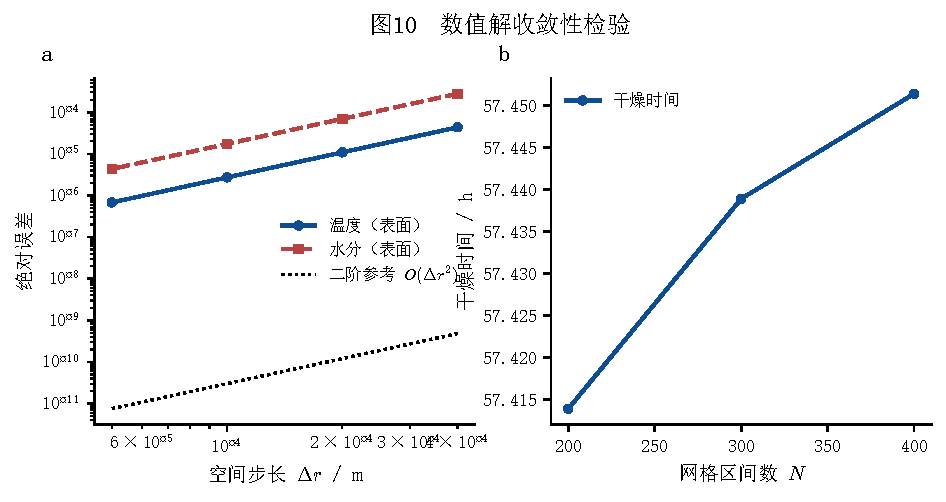
\includegraphics[width=0.98\textwidth]{texfile/figures/fig10_convergence.pdf}
	\caption{数值解收敛性检验（a：问题一空间误差；b：问题三烘干时间收敛）}
	\label{fig:convergence}
\end{figure}

\subsection{质量守恒检验}

控制体积格式天然满足通量守恒。以问题三为例，对整个干燥过程做干基水分质量衡算：初始水分 $100\%$，其中\textbf{预热段（0--4 h）蒸发去除 $55.5\%$、恒温段蒸发去除 $39.7\%$、结束时残留 $4.8\%$}，三者合计 $100\%$，水分质量严格守恒（图~\ref{fig:sankey}）。这从物理上验证了模型与数值格式的正确性。

\begin{figure}[htbp]
	\centering
	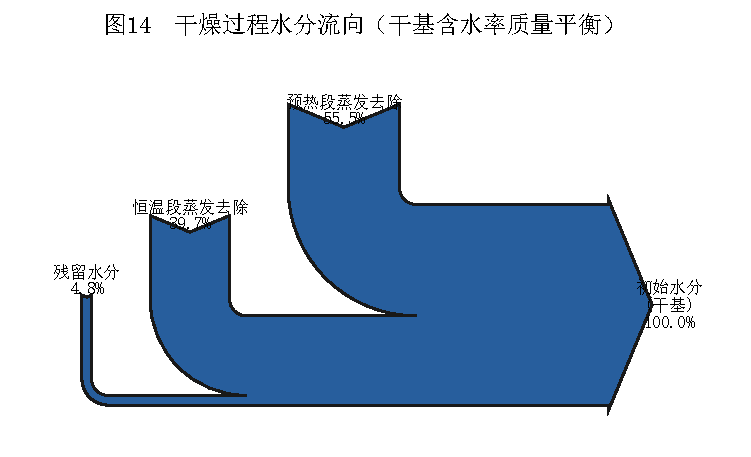
\includegraphics[width=0.78\textwidth]{texfile/figures/fig14_sankey.pdf}
	\caption{干燥过程水分流向（Sankey 图）}
	\label{fig:sankey}
\end{figure}

\subsection{灵敏度分析}

为评估参数不确定性对结果的影响，以问题三为基准，将各参数分别扰动 $\pm20\%$，考察烘干结束时间的变化，结果如表~\ref{tab:sensitivity} 与图~\ref{fig:sensitivity} 所示。

\begin{table}[htbp]
	\caption{参数 $\pm20\%$ 对干燥时间的影响（基准 $57.33$ h）}
	\label{tab:sensitivity}
	\centering
	\begin{tabular}{lccc}
		\toprule
		参数 & $-20\%$ 时干燥时间/h & $+20\%$ 时干燥时间/h & 影响程度 \\
		\midrule
		半径 $R_0$ & 37.83 & 80.95 & 最显著 \\
		烘房温度 $T_{air}$ & 80.30 & 42.63 & 显著 \\
		对流传质系数 $h_m$ & 59.05 & 56.27 & 较显著 \\
		初始含水率 $C_0$ & 56.25 & 58.18 & 较显著 \\
		空气湿度 $C_{air}$ & 57.07 & 57.65 & 较小 \\
		对流换热系数 $h$ & 57.35 & 57.32 & 可忽略 \\
		\bottomrule
	\end{tabular}
\end{table}

\begin{figure}[htbp]
	\centering
	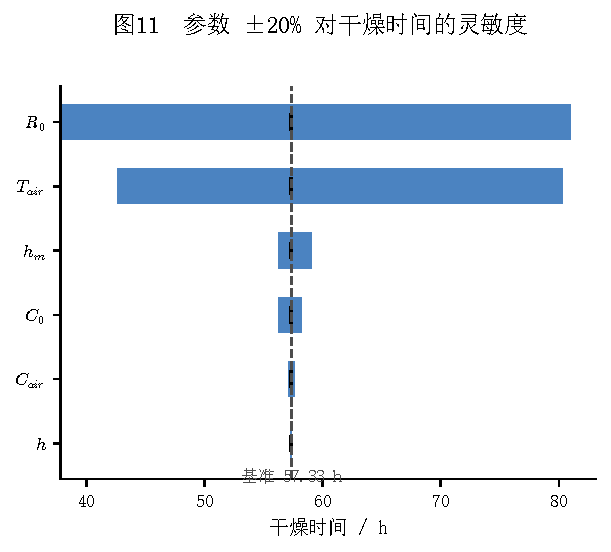
\includegraphics[width=0.62\textwidth]{texfile/figures/fig11_sensitivity.pdf}
	\caption{参数 $\pm20\%$ 对干燥时间的灵敏度（tornado 图）}
	\label{fig:sensitivity}
\end{figure}

结果表明：半径 $R_0$ 与烘房温度 $T_{air}$ 对干燥时间影响最为显著——干燥时间近似正比于 $R^2$，而扩散系数 $D$ 随温度呈 Arrhenius 型指数变化（$D\propto e^{-3850/T}$），故提高烘房温度可大幅缩短干燥周期；对流传质系数 $h_m$ 与初始含水率 $C_0$ 次之；空气湿度 $C_{air}$ 与对流换热系数 $h$ 影响很小。这提示工程上应优先控制烘房温度与药材尺寸，并保证足够的表面通风（增大 $h_m$）。

为进一步量化各参数对干燥时间的\textbf{贡献度}，以拉丁超立方抽样生成 60 组参数样本，计算对应干燥时间并拟合随机森林代理模型，进而采用 SHAP 方法 \cite{lundberg2017unified} 计算各参数的贡献度，结果如图~\ref{fig:shap} 所示。SHAP 分析给出的参数重要性排序为：$R_0 > T_{air} > h_m > C_0 > C_{air} > h$，与单因素灵敏度分析结论一致，验证了分析结果的稳健性。

\begin{figure}[htbp]
	\centering
	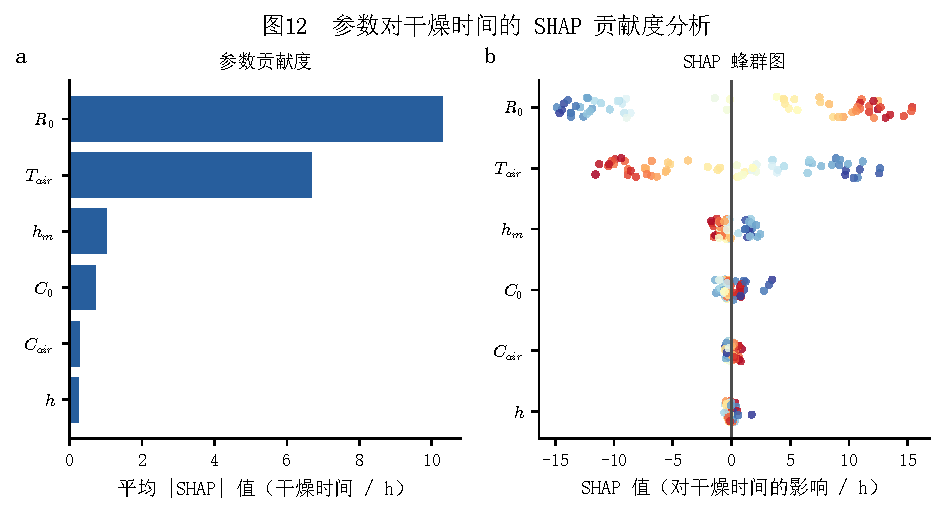
\includegraphics[width=0.98\textwidth]{texfile/figures/fig12_shap.pdf}
	\caption{参数对干燥时间的 SHAP 贡献度分析（a：平均贡献度；b：蜂群图）}
	\label{fig:shap}
\end{figure}
